\documentclass[conference]{IEEEtran}
\usepackage{amsmath,amsfonts,amssymb}
\usepackage{graphicx}
%\usepackage{caption}
\usepackage{subfig}
\usepackage{color}

%\usepackage{url}

\begin{document}
\title{CS8803-O03 Reinforcement learning\\Project 3 report}

\author{\IEEEauthorblockN{Rohan D. Kekatpure}
\IEEEauthorblockA{Email: rdk@gatech.edu}}
% make the title area
\maketitle

% As a general rule, do not put math, special symbols or citations
% in the abstract
%\begin{abstract}
%\end{abstract}

\IEEEpeerreviewmaketitle
\section{Introduction}
Multi-agent Q-learning is a nontrivial departure from regular (deterministic action, single $Q$ function) Q learning in two ways: (1) state values are functions of multiple Q's (2) optimal policies are allowed to be stochastic. The Greenwald paper \cite{greenwald} demonstrates the inadequacy of regular Q learning and convergence of multi-agent Q learning learning. Project 3 aims to deepen our understanding of multi-agent (adversarial or cooperative) Q learning through reproduction of Greenwald's results for a $2\times4$ grid game called soccer.

%%
\section{Quick theory tour}
The paper presents four multi-agent Q learning options:
\begin{enumerate}
\item {\bf Regular:} Ignore the opponent's $Q$ function and actions. Agents are only coupled through rewards. The policy is deterministic and $Q$ function at each state for each agent is simply a vector of $n$ values ($n=5$ in our case). The state value is the max for $Q_i$: 
\begin{equation}
V_i =\max_{a\in A_i} Q_i(s,a)
\end{equation} 
%
\item {\bf Friend Q: } Ignore the opponent's $Q$ function, but consider its actions. Optimal policy is deterministic, and $Q$ function at each stage is a $n\times n$ matrix. The value for each state is the max across this matrix:
\begin{equation}
V_i = \max_{\vec{a}\in A_1\times A_2} Q_i(s, \vec{a})
\end{equation}
%
\item {\bf Foe Q: } Ignore opponent $Q$ function, consider its actions, but calculate the value function using {\bf maximin} instead of simple max. This requires linear programming (LP). Maximin also allows {\bf stochastic} optimal policies represented as a probability distribution over $n$ action values. The $Q$ is an $n\times n$ matrix and the state value is: 
%
\begin{equation}
V_i = \max_{\pi\in\text{PD}(A)}\min_{o\in O}\sum_{a\in A}\pi_a Q_i(s, a, o)
\end{equation}
%
\item {\bf CE Q: } Consider joint actions and compute state value as a function of agents' $Q$ values
%
\begin{equation}
V_i = f_i(Q_1, Q_2)
\end{equation}
where the functions $f_i$ are linear combinations of $Q_i$ and determined through linear programming. 
\end{enumerate}
%%
\section{Implementation methodology}
\subsection{Overview}
%%
\subsection{Software dependencies}
%%
\section{Experiments}
%
\begin{figure*}
\begin{tabular}{cc}
    \subfloat[CE-Q] {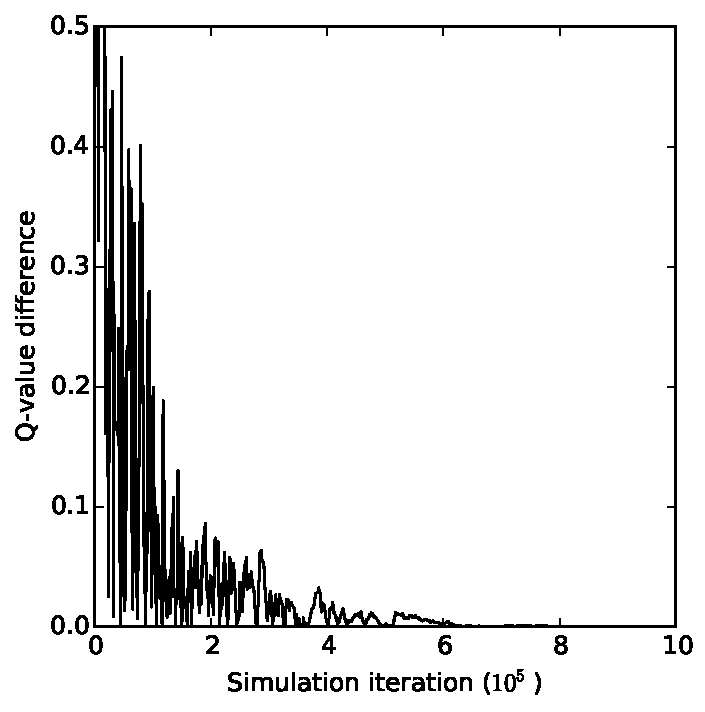
\includegraphics[width=0.45\textwidth]{./figures/ceq.pdf}} 
    & \subfloat[Foe-Q] {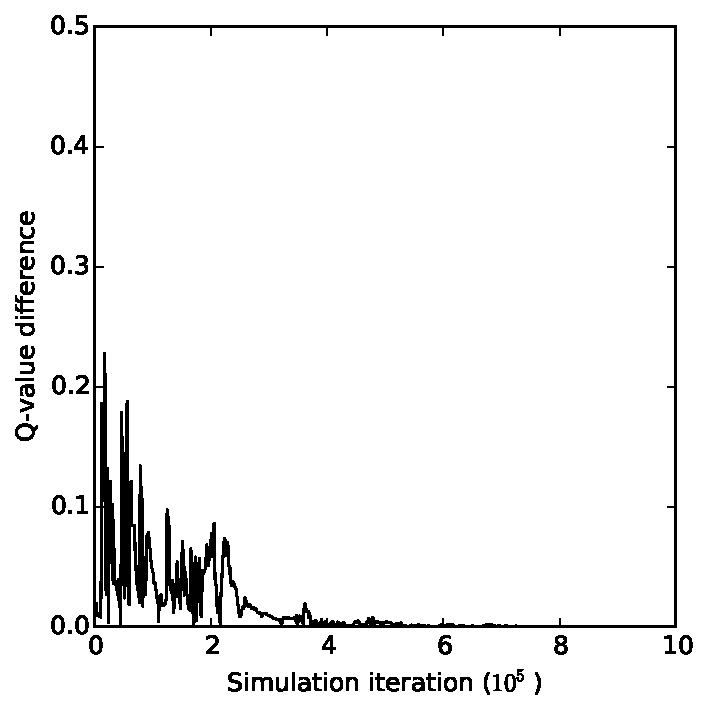
\includegraphics[width=0.45\textwidth]{./figures/foe.pdf}} \\
    \subfloat[Friend-Q] {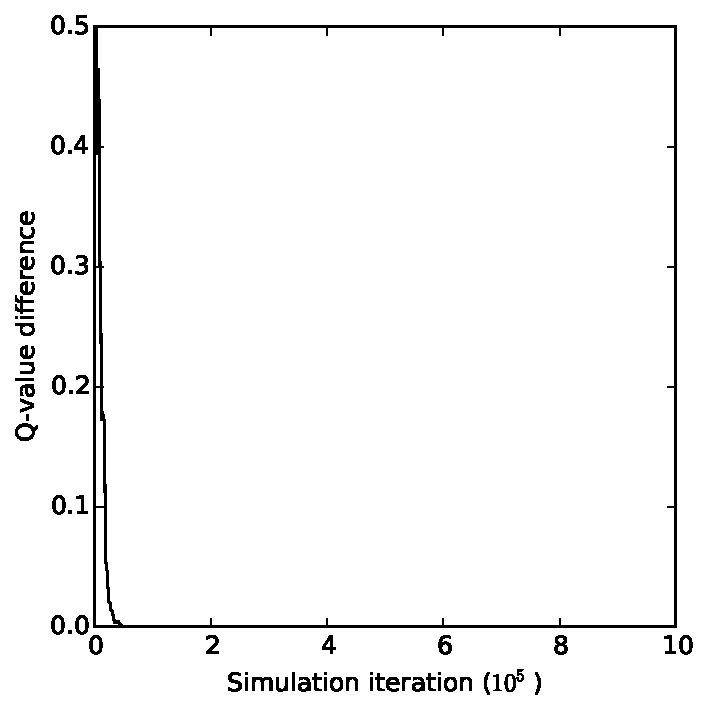
\includegraphics[width=0.45\textwidth]{./figures/friend.pdf}}
    & \subfloat[Q-learning] {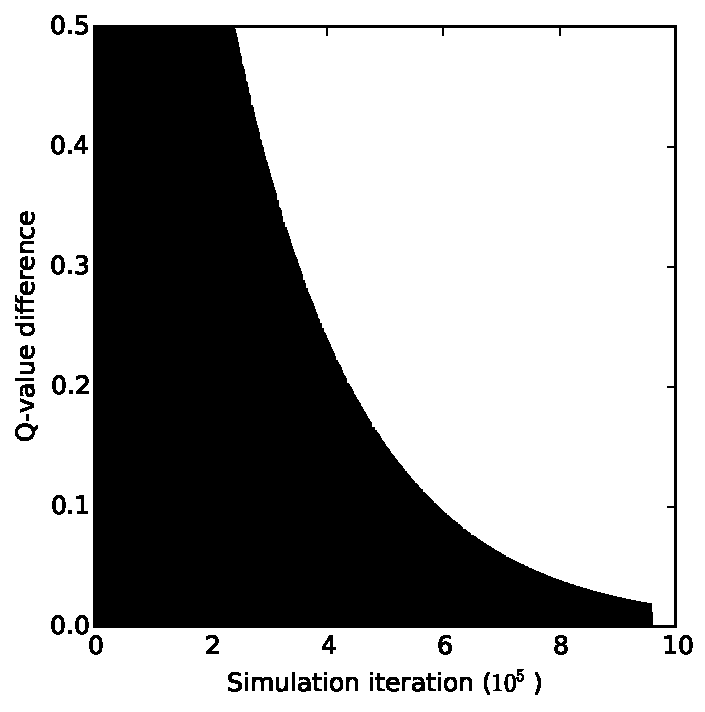
\includegraphics[width=0.45\textwidth]{./figures/qlearning.pdf}}    
\end{tabular}
\end{figure*}
%%
\section*{Summary}
\begin{thebibliography}{1}
\bibitem{greenwald}
A.~Greenwald and K.~Hall, ``Correlated Q learning,'' {\em ICML}, 2001.
\end{thebibliography}

\end{document}


